\documentclass[twocolumn]{article}

\usepackage{color}
\usepackage[margin=1in,bottom=1.5in]{geometry}

\usepackage{graphicx}
\usepackage{subcaption}

% Comment out second line to disable.
% Thanks: https://gist.github.com/orbekk/1298622
\newcommand{\todo}[1]{}
\renewcommand{\todo}[1]{{\color{red} TODO: {#1}}}

\newcommand{\secref}[1]{Section~\ref{sec:#1}}
\newcommand{\seclab}[1]{\label{sec:#1}}
\newcommand{\figref}[1]{Figure~\ref{fig:#1}}
\newcommand{\figlab}[1]{\label{fig:#1}}
\newcommand{\tblref}[1]{Table~\ref{tbl:#1}}
\newcommand{\tbllab}[1]{\label{tbl:#1}}

\title{Modeling Image Segmentation as Epidemic Spread in an Interdependent Network}
\author{
  Connor Greenwell, Emory Hufbauer\\
  Computer Science Dept. \\
  University of Kentucky
}
\date{}

\begin{document}

\maketitle

\begin{abstract}
In this document we propose formulating the problem of image segmentation as
simulating the propagation of information/ownership through an interdependent
network where the first layer is a lattice representation of an input image and
the second layer is a (planar) overlay graph where each node has weighted edges
to pixels in the lattice. We design and evaluate a number of propagation
models, primarily based on pixel/region similarity metrics. Finally we 
compare our method against classical and current state-of-the-art methods for
image segmentation on a variety of segmentation benchmark datasets. 
\end{abstract}

\section{Introduction}

Instance segmentation is an important and popular topic in computer vision
\cite{newell2017associative, li2017fully, ren2017end}.   It is important to note
that instance segmentation is a distinct but related task to object detection.
Notably, instance segmentation is not concerned with \emph{what} and object
is, only \emph{where} it is. Typically this is formulated as assigning a
unique label to each pixel in an image, where the label indicates belonging to a
particular object. For example, an object containing two cats would have three
labels: one for each cat, and a background label. Current state of the art uses
convolutional neural networks to segment an image into its consituent object
parts.

Interdependent graphs are a tool commonly used for analyzing cyber-physical
networks and social networks. They are represented by a pair of distinct graphs
joined with some number of interdependency links between nodes in each graph.
We propose a method based on the epidemic spread of information through an
interdependent graph.

We first create an interdependent network model of an image. The
weights of edges between adjacent pixels in the lattice represent
their degree of similarity to each other. The weights of edges between
nodes in the overlay graph represent their overlap and estimated
potential to belong to the same object. The weights of edges between the
overlay and lattice represent ownership of pixels by superpixels.
We then perform a simultaneous, competitive propagation of multiple
phenomena through this network using a variety of models, with the
ultimate goal of developing a propagation model with property that,
after propagation has completed, the regions of the lattice affected by
each phenomena correspond well to the segments of the image.

The following paper is layed out as follows: In \secref{related} we survey the
current state of the art in image segmentation, as well as methods related to
ours. In \secref{approach} we describe our method in detail. In \secref{eval} we
describe the metrics by which we judge our methods and those we compare against.
In \secref{data} we describe the benchmark datasets against which we compare.
Finally, in \secref{results} we describe our resulting performance and
evaluation.

\section{Related Work}\seclab{related}

\todo{endemic spread in interdpenedent networks}

\todo{image segmentation: classic, modern, and weird methods}
\cite{pei2014saliency} use a Markov-Random-Field on precomputed super pixels to
perform image segmentation.  \cite{newell2017associative,li2017fully,ren2017end}
present a variety of neural network based approached to instance segmentation on
natural images.

\begin{figure*}[t]
\centering

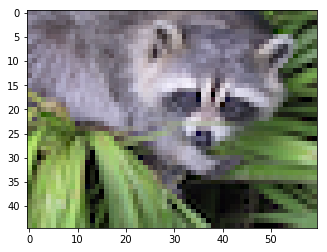
\includegraphics[width=0.3\linewidth]{figs/input.png}
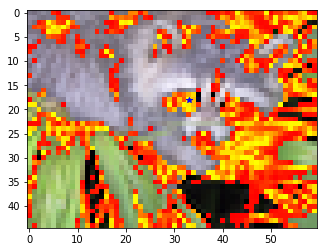
\includegraphics[width=0.3\linewidth]{figs/alpha.png}
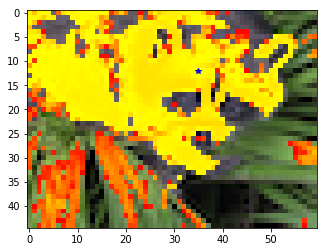
\includegraphics[width=0.3\linewidth]{figs/beta.png}

\caption{
(left) A sample image from our dataset.
(middle) The inverse square of the difference between every pair of pixels in
the image. 
(right) Transformation of the color space to the median centroid of the image's
profile, projected onto the surface of a sphere in color space, points on the
surface of which represent unique, continuous, colors. The cosine of the angular
distance between each pair of pixels on the sphere.
(middle), and (right) are used to determine epidemic spread probabilities
between pixels in our approach.
}
\figlab{alpha_beta}
\end{figure*}

\section{Approach}\seclab{approach}

First we encode an input image as a pair of identical graphs where each node is
represents a pixel, and edges represent adjacency between pixels in the image.
We create an interdependent network model of an image. The weights of
edges between adjacent pixels in each graph represents their degree of
similarity to each other, which we describe in the next subsection. Since pixels
are represented by nodes in both graphs, we connect their respective nodes with
an interdependency link with a uniform weight.

We then perform a simultaneous, competitive propagation of multiple
phenomena through this network using a variety of models, with the ultimate goal
of developing a propagation model with property that, after propagation has
completed, the regions of the lattice affected by each phenomena correspond well
to the segments of the image. This produces a proposal segmentation for each
image pixel, which is defined as a per-pixel likelyhood of belonging to the same
object as the source pixel.

Finally, each proposed segmentation is thresholded to produce a binary mask
which we combine with a naive segmentation merging algorithm which iteratively
applies a logical OR to each successive pair of proposed segmentations. 

\subsection{Image Network Extraction}

As a preprocessing step we extract two meaningful metrics from the pixels of an
input image and use them to define similarity scores between adjacent pixels.
\todo{maybe emory can ellaborate on this here}
The first is extracting value information from the image.
The approach takes the inverse square of the difference between every pair of
pixels in the image. 

The other method is extracting the hue data. This complements the value method
nicely.  First, we transform the color space to the median centroid of the
image's profile. We then compute the norm of each pixel in the image,
post-transform.  Next, we take the dot product of every pair of pixels, and
finally normalize against each via the norms recorded before.  Intuitively, it's
transforming the (0,0,0)->(1,1,1) cube of RGB color space to a hollow sphere
centered at the origin, points on the surface of which represent unique,
continuous, colors. We then output the cosine of the angular distance between
each pair of pixels on the sphere as a 4D structure like above.

The result of each approach is a four-dimensional array or "image of
images", which we visualize in \figref{alpha_beta}.

\begin{figure}
  \centering
  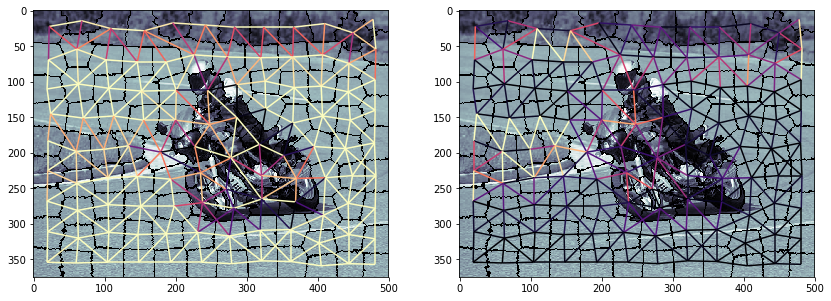
\includegraphics[width=\linewidth]{figs/ab_graphs.png}

  \caption{
    The original overlay graphs on a sample image. In each, lighter colors represent higher scores; best viewed in color.
    (left) alpha scores, based on color intensity. (right) beta scores, based on hue difference.
  }
  \figlab{ab_graph}

\end{figure}

\begin{figure*}[t]
  \centering

  \begin{subfigure}{0.49\linewidth}
    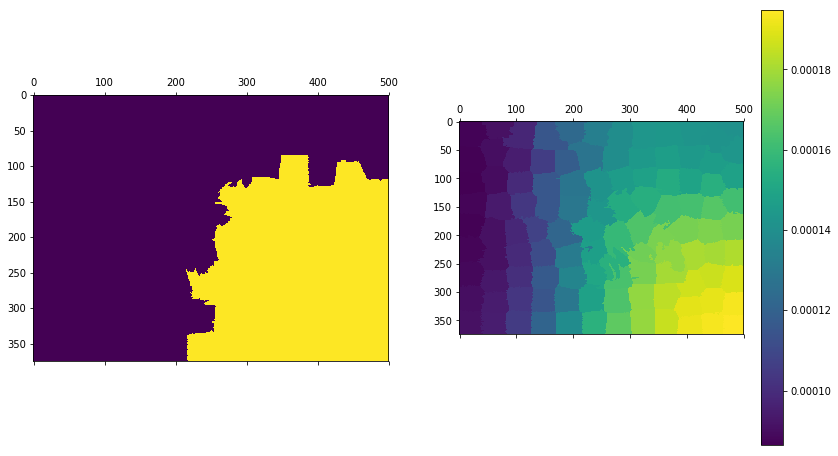
\includegraphics[width=\linewidth]{figs/single_source.png}
    \caption{Probability distribution over superpixels.}
  \end{subfigure}
  \begin{subfigure}{0.49\linewidth}
    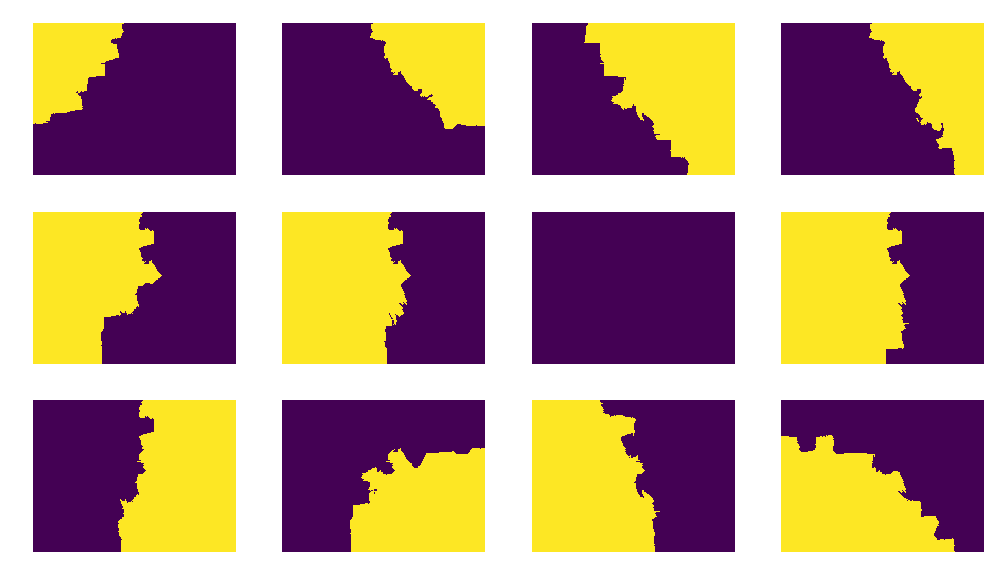
\includegraphics[width=\linewidth]{figs/many_sources.png}
    \caption{Binary masks for various source regions.}
  \end{subfigure}
  \begin{subfigure}{0.49\linewidth}
    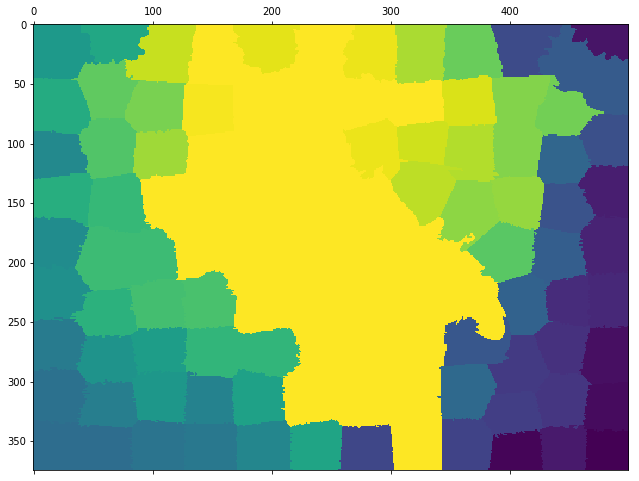
\includegraphics[width=\linewidth]{figs/aggregate.png}
    \caption{Aggregate of many binary masks. \todo{This is REALLY bad. I must be doing something wrong\ldots}}
  \end{subfigure}
  \begin{subfigure}{0.49\linewidth}
    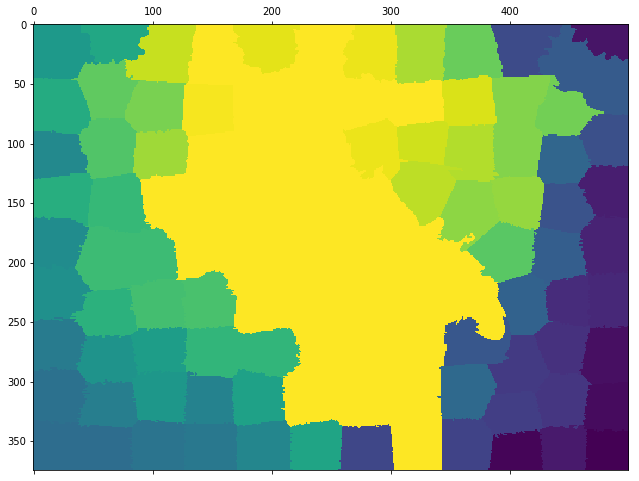
\includegraphics[width=\linewidth]{figs/aggregate.png}
    \caption{\todo{replace this with something else! maybe g.t. segmentation}}
  \end{subfigure}

  \caption{
    Overview of our method: First, a \todo{blarg}
  }
  \figlab{process}

\end{figure*}

\subsection{Baseline}

A naive baseline method has been developed for us to compare our actual method
against. It is based on using DBSCAN \cite{ester1996density} to cluster and
merge superpixels produced by SLIC \cite{achanta2010slic}.

\section{Evaluation}\seclab{eval}


As a preprocessing step, we pre-segment each image into superpixels using the
SLIC-Zero parameter-free superpixelization method \cite{achanta2010slic}. We
hypothesisize that this does not significantly degrade our results. 

The goal of this project is mostly to explore the space and point to future
research possibilities. Although the results are compared with those of
existing algorithms, they are not expected to be competitive with the state of
the art. To that end we evaluate our performance on a classic image segmentation
benchmark dataset, PASCAL VOC, which contains $2,913$ full resolution images and
per-pixel instance segmentations.

We evaluate our methods on the Adjusted Rand Score from
\cite{unnikrishnan2005measure}.  

We evaluate two different methods for simulating information propagation in our
proposed interdependent graph. The first is based on random walks which we
simulate with Markov chains. We experiment with different walk horizons. The
second is based on an approximation of epidemic spread. \todo{Emory, please
explain this in detail here.}

\subsection{Dataset}\seclab{data}

The dataset upon which we evaluate our method is the PASCAL Visual Object
Classification (VOC) dataset \cite{Everingham10}. Over the years in which the
VOC challenge was run, a couple different variations of the problem we
presented, ranging from whole-image object classification to human pose
estimation. In 2012 they introduced a subset of per-pixel instance segmentations
for $2,913$ of the images in the dataset. In each segmentation, there is a
background class, some number of instance classes, and a "don't care" region
around each object instance. The instance segmentation task is distinct from
object classification in that the goal is not to actually classify to which
object category each pixel belongs to, but to separate the image into its
constituent parts, similar to foreground/background segmentation. We believe
that this task presents a unique challenge that can be addressed by our proposed
method of propagating information through a interdependent graph defined by
pixel/region similarities.

\section{Results}\seclab{results}

\begin{figure}[t!]
\centering

  \begin{subfigure}{\linewidth}
    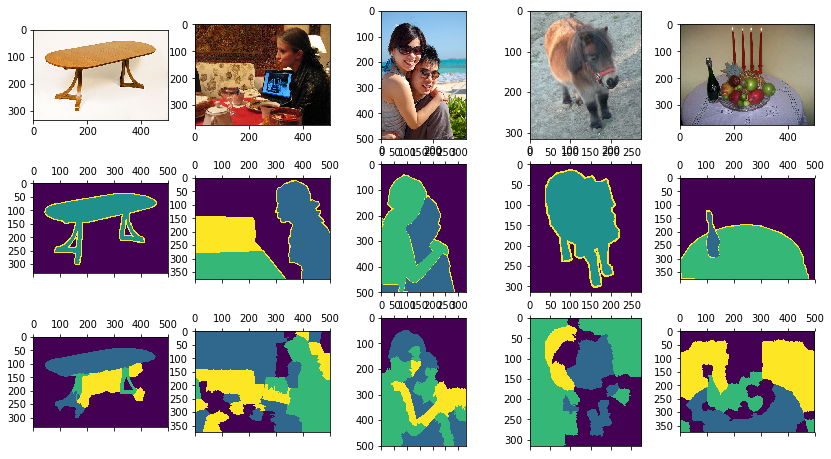
\includegraphics[width=\linewidth]{figs/baseline_best.png}
    \caption{Baseline}
  \end{subfigure}

  \begin{subfigure}{\linewidth}
    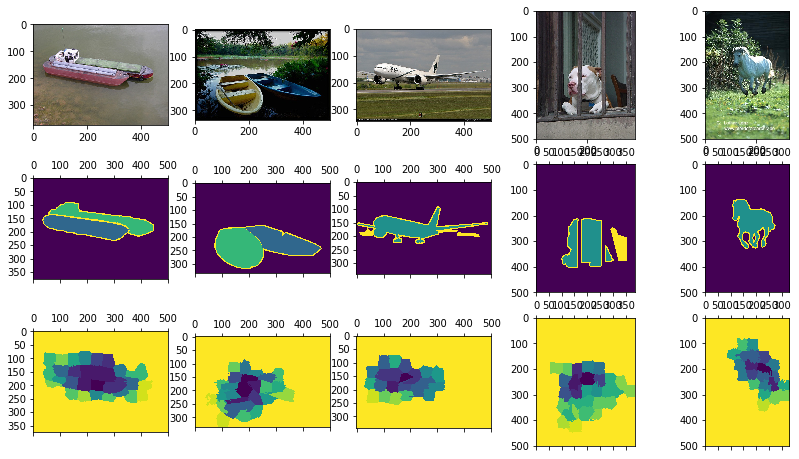
\includegraphics[width=\linewidth]{figs/markov_best.png}
    \caption{Markov random walk based}
  \end{subfigure}

  \begin{subfigure}{\linewidth}
    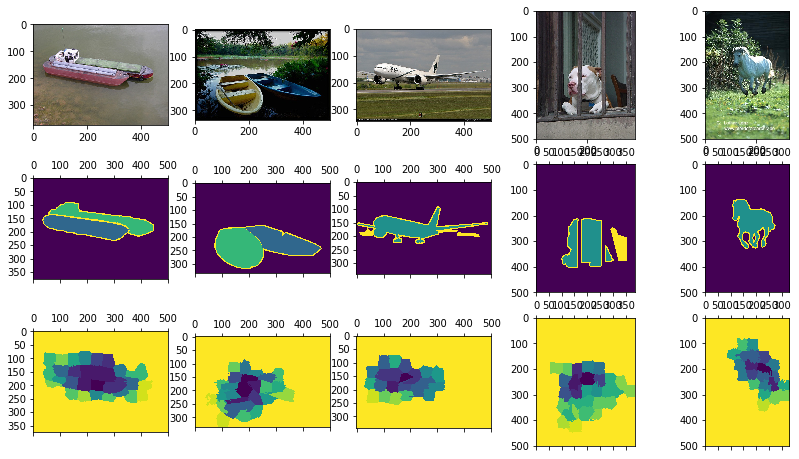
\includegraphics[width=\linewidth]{figs/markov_best.png}
    \caption{\todo{Epidemic based}}
  \end{subfigure}

\caption{Sample results from each of our proposed methods.}
\end{figure}

\begin{figure}
  \centering

  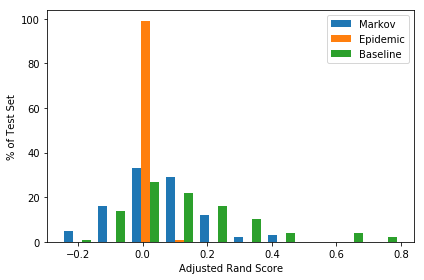
\includegraphics[width=\linewidth]{figs/bars.png}

  \caption{Comparison of Adjusted Rand Score on 100 images from the training set. Having more area to the right of the graph
indicates a higher proportion of high quality seqmentations. In this case, this indicates that our method is worse than our
defined baseline.
  }
  \figlab{bars}

\end{figure}

\begin{figure*}[t]
  \centering

  \begin{subfigure}{0.49\linewidth}
    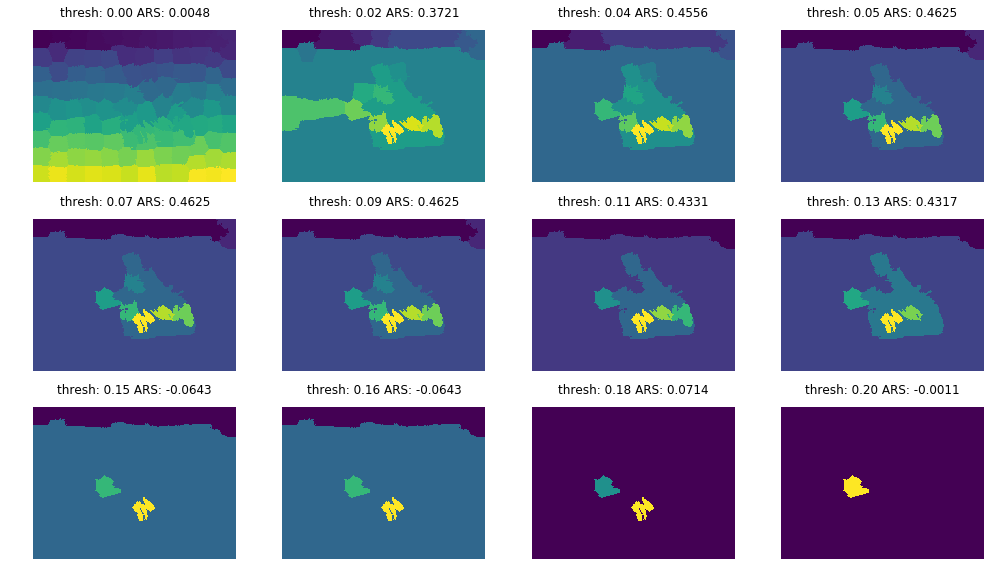
\includegraphics[width=\linewidth]{figs/only_alpha.png}
    \caption{Sample segmentation using only the alpha scores.}
  \end{subfigure}
  \begin{subfigure}{0.49\linewidth}
    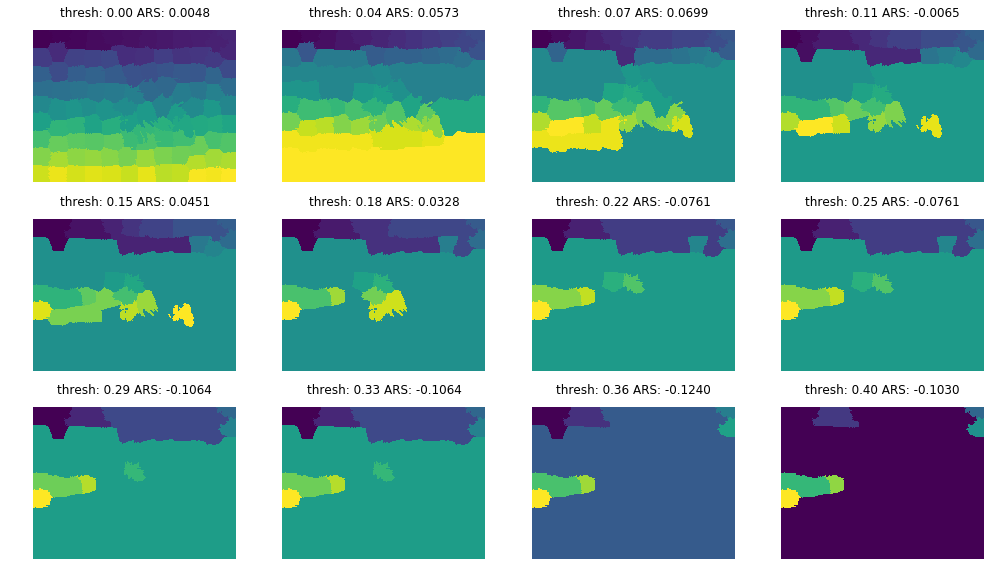
\includegraphics[width=\linewidth]{figs/only_beta.png}
    \caption{Sample segmentation using only the beta scores.}
  \end{subfigure}

  \caption{
    \todo{foobar}
  }
  \figlab{ab_only}

\end{figure*}

\todo{This section should be a boat load of tables and plots. Hopefully we look good in some of them}

\todo{
Mechanisms for performing hyperparameter optimization have been developed and tested on the naive baseline. This will be
necessary because our final method will likely have a number of tunable hyperparameters and it will be useful to automatically
find the optimal settings for our task.
}

\begin{figure*}[t!]
  \centering

  \begin{subfigure}{0.49\linewidth}
    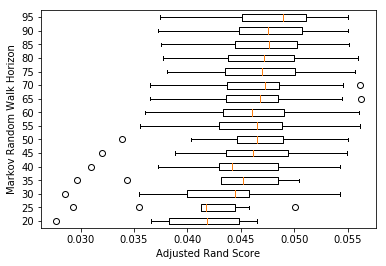
\includegraphics[width=\linewidth]{figs/markov_horizon.png}
    \caption{Markov random walk, walk horizon}
  \end{subfigure}
  \begin{subfigure}{0.49\linewidth}
    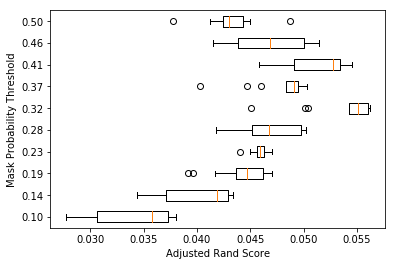
\includegraphics[width=\linewidth]{figs/markov_thresh.png}
    \caption{Markov random walk, merge threshold}
  \end{subfigure}

  \begin{subfigure}{0.49\linewidth}
    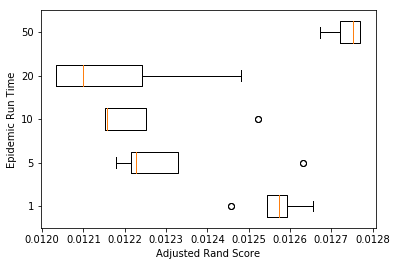
\includegraphics[width=\linewidth]{figs/epidemic_run.png}
    \caption{Epidemic, simulation runtime}
  \end{subfigure}
  \begin{subfigure}{0.49\linewidth}
    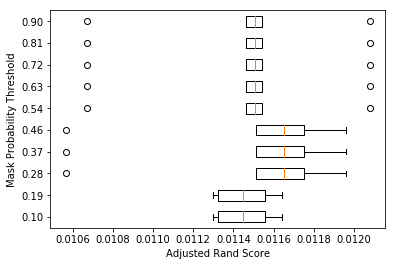
\includegraphics[width=\linewidth]{figs/epidemic_thresh.png}
    \caption{Epidemic, merge threshold}
  \end{subfigure}

  \caption{
    Analysis of performance under different hyperparameters for each of our proposed methods. (a) and (b) show that threshold
    is the most important parameter. \todo{bottom row should be for epidemic model}
  }
  \figlab{ab_only}

\end{figure*}

\section{Conclusion}

In this document we presented a method for performing instance segmentation on photographs by modeling instance membership as
an information spread or epidemic model in an interdependent graph. We introduced two simple similarity metrics which are used
as the basis for tranmitting instance membership between neighboring pixels. Finally we compare our method to a rudamentary
baseline.

\subsection{Future Work}

Our method is easy to extend. Some possible directions for future work include the following:

\begin{itemize}
  \item Improving the method by which we combine candidate segmentations.
  \item Incorporating additional similarity metrics, and additional layers to the interdependent graph.
  \item Explore the effect of using other superpixel segmentation strategies.
\end{itemize}

\bibliographystyle{plain}
\bibliography{refs} 

\end{document}
